\documentclass[11pt]{article}
\usepackage[margin=1in]{geometry}
\usepackage{fontspec}
\usepackage{ucharclasses}
\usepackage{graphicx}
\usepackage{booktabs}
\usepackage{array}
\usepackage{hyperref}
\usepackage{enumitem}
\usepackage{titlesec}

\defaultfontfeatures{Ligatures=TeX}
\setmainfont{TeX Gyre Termes}
\newfontfamily\hangulfont[ItalicFont={Noto Sans CJK KR}]{Noto Sans CJK KR}
\setTransitionsForCJK{\hangulfont}{}{}

\setlength{\parskip}{0.5em}
\setlength{\parindent}{0pt}
\titleformat{\section}{\large\bfseries}{}{0em}{}
\titleformat{\subsection}{\normalsize\bfseries}{}{0em}{}

\title{Selective Refinement Status Report}
\author{Internal Research Note}
\date{2026-04-09}

\begin{document}
\maketitle

\section{Executive Summary}

현재 양성 결과는 존재한다. 그러나 그 결과가 입증하는 범위는 좁다. two-pass 계열 selective refinement는 bounded NIAH에서 retrieval recovery signal을 보였지만, 현재 스크립트는 저장된 KV cache 자체를 low-bit representation으로 바꾸지 않는다. 따라서 이 결과는 compressed-cache method가 아니라 attention-path proxy diagnostic으로만 해석해야 한다.

\section{Verified Facts}

\begin{tabular}{>{\raggedright\arraybackslash}p{0.28\linewidth} >{\raggedright\arraybackslash}p{0.64\linewidth}}
\toprule
Item & Verified result \\
\midrule
Mistral 4K same-harness & \texttt{baseline\_2bit=0.333}, \texttt{two\_pass\_k16=1.000}, best \texttt{query\_dequant=0.333}, all \texttt{sharp\_temp=0.000}. \\
4K two-pass sweeps & Mistral and Qwen both saturate at \texttt{k=8,16,32,64} with score \texttt{1.000}. \\
Proxy selective promotion & Mistral 4K proxy smoke gives \texttt{uniform\_2bit=0.000}, \texttt{uniform\_3bit=0.667}, \texttt{cliffkv\_k64\_b3=1.000}, \texttt{avg\_bits\_per\_dim=2.016}. \\
QDRP & Synthetic budget-1 helps, but budget-2 pure risk fails and hybrid is nearly neutral. \\
TRIC & Recursive predictor improves over copy-last but loses to shared linear in every tested synthetic setting. \\
\bottomrule
\end{tabular}

\section{What Is Invalid To Claim}

The current scripts explicitly state that the underlying KV cache remains FP16 and that low-bit logic is applied only on the attention path. That single implementation fact blocks any honest claim about stored cache size, true HBM savings, or storage-valid mixed-precision KV compression.

Accordingly, the following claims are not allowed:
\begin{itemize}[leftmargin=1.5em]
\item ``This is already a storage-valid KV-cache compression method.''
\item ``The current effective average bit numbers are fair stored-cache budgets.''
\item ``Two-pass selective refinement is already ready as a paper method.''
\end{itemize}

\section{Direction-Level Verdict}

\subsection{Two-Pass Selective Refinement}

This direction stays alive, but only as a diagnostic program. Its strength is the size and consistency of the NIAH recovery signal. Its weakness is that the current implementation is still a proxy harness and that 4K bounded NIAH is already saturated.

\subsection{QDRP}

This direction should be held, not advanced. The theoretical framing is still interesting, but the current empirical evidence does not justify more GPU beyond a revised real-trace risk calibration.

\subsection{TRIC}

This direction should be stopped for now. Losing to a shared linear predictor in synthetic diagnostics is enough to rule out immediate end-to-end investment.

\section{Next Plan}

The next step is not a new method. It is a narrower test of the current positive signal.

\begin{itemize}[leftmargin=1.5em]
\item Run selector diagnostics: \texttt{two\_pass} vs \texttt{recent\_k}, \texttt{sink\_k}, \texttt{random\_k}.
\item Run harder frontiers at 8K and 16K with \texttt{k=1,2,4,8,16}.
\item If the signal survives, rewrite the method into a storage-valid cache path before making any compression claim.
\end{itemize}

\section{Figures}

\begin{figure}[h]
\centering
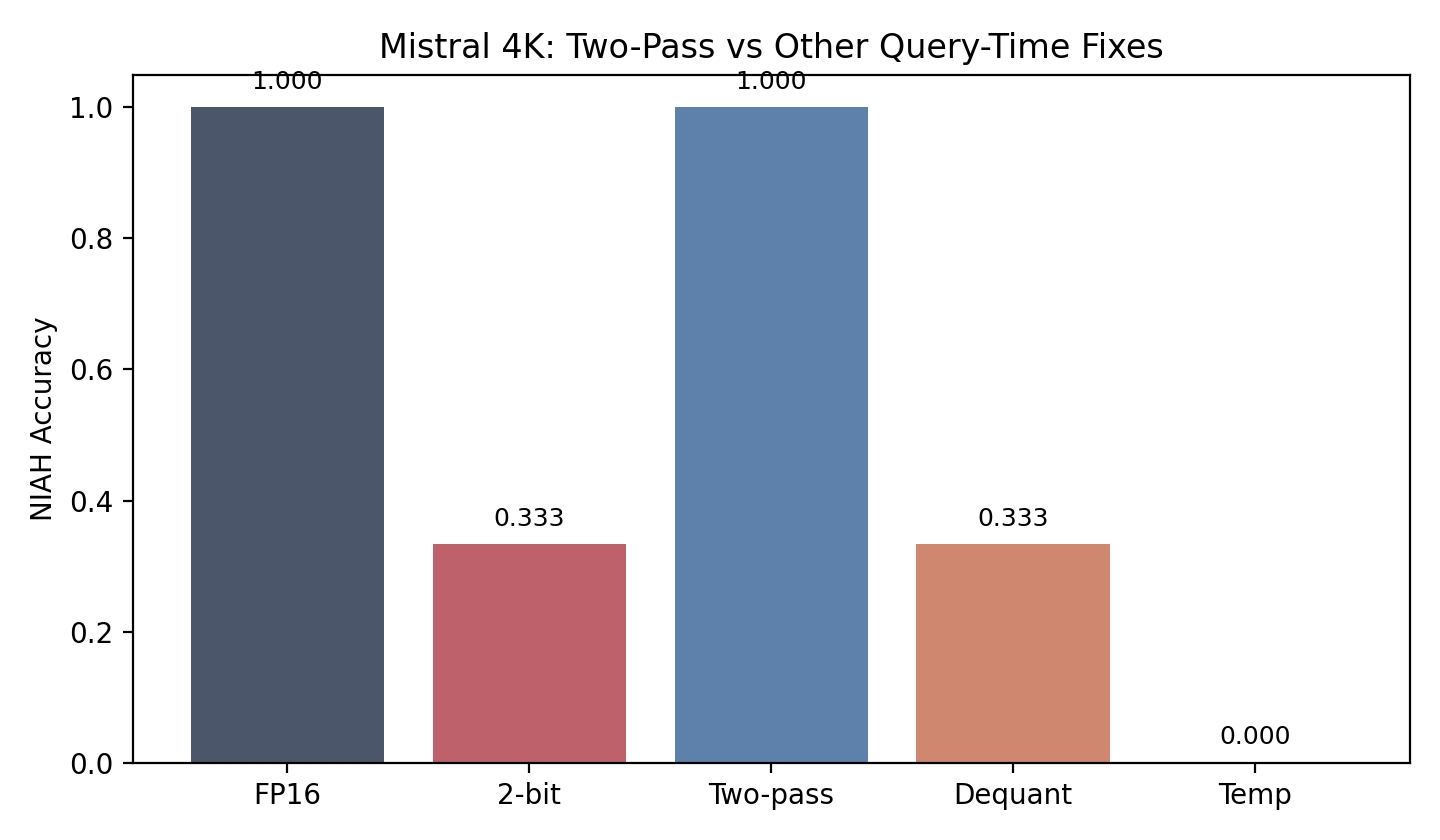
\includegraphics[width=0.82\linewidth]{figures/selective_refine_mistral_method_compare.png}
\caption{Same-harness Mistral 4K comparison. Only \texttt{two\_pass} clearly beats the 2-bit baseline on the current proxy harness.}
\end{figure}

\begin{figure}[h]
\centering
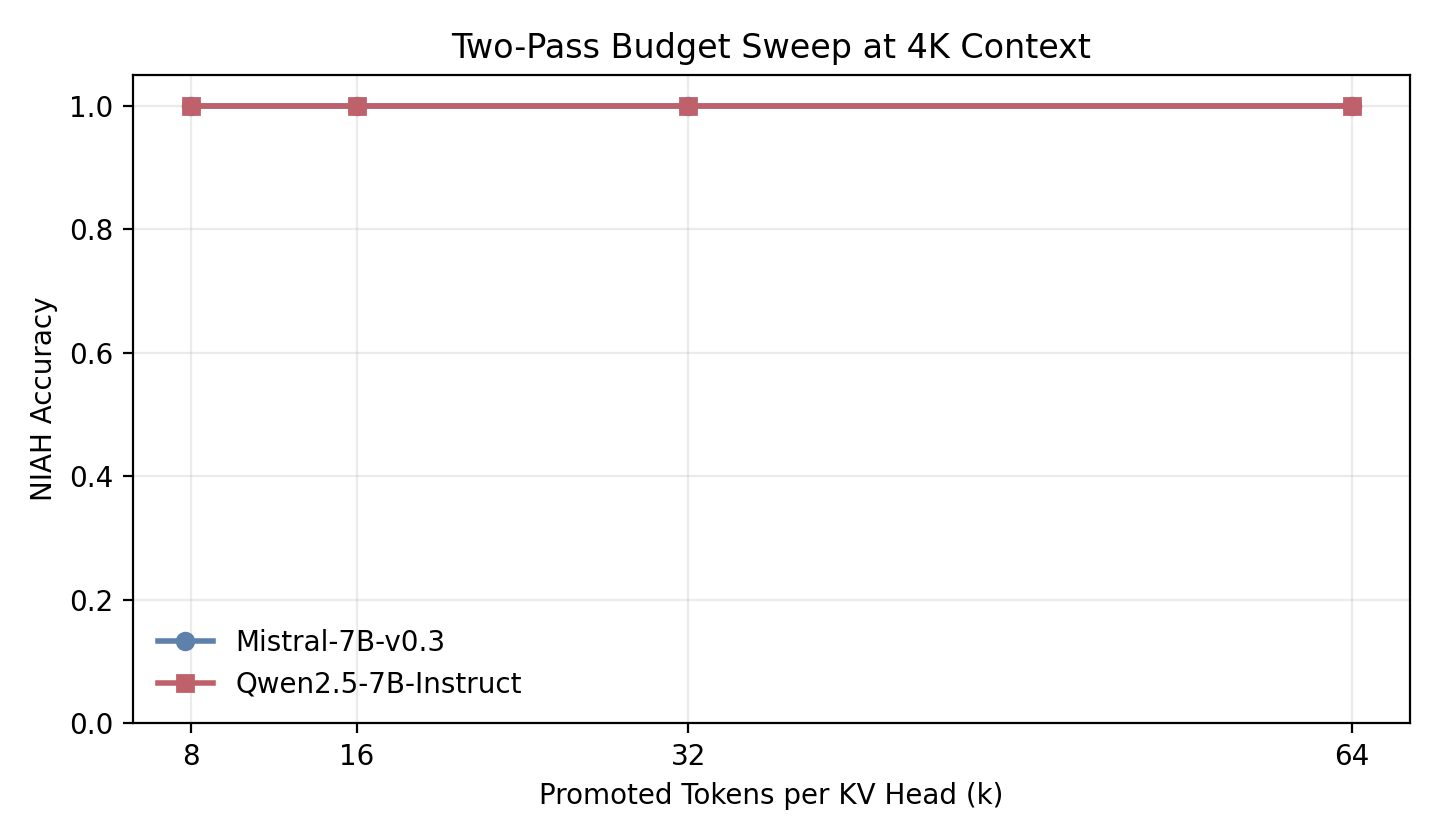
\includegraphics[width=0.82\linewidth]{figures/selective_refine_two_pass_budget_sweep.png}
\caption{4K two-pass sweep. The grid is saturated, so it demonstrates a positive signal but not the true minimum-budget frontier.}
\end{figure}

\end{document}
